\section{Literature Review}
Through this literature review we aim to summarise the key methodologies in mixed-precision Monte Carlo methods in the literature that are relevant to our work. In this report we work to understand how we can utilise and exploit reconfigurable hardware with mixed-precision to take advantage of unique features in the computing architectures of FPGAs over GPUs. We perform this research within the context of Mathematical Biology in which large quantities of statistical independent simulations are required to produce meaningful results. This presents a clear use case for these methods as there is potential for both the wall-time and power efficiency improvements over conventional computing frameworks. 

\subsection{Heterogeneous Computing}\label{sec:heterogeneous_computing}
It is important to first understand heterogeneous computing as a framework to conceptualise how reconfigurable and accelerator hardware can be used to complement and improve existing computing ecosystems. Heterogeneous computing environments are those in which there are multiple different computer architectures, primarily central processing units (CPUs) and graphical processing units (GPUs). By doing this, we can allocate tasks in our program to these specific devices depending on the type of operations that are being done on them. 

This key advantage provided by conducting our computations in a heterogeneous environment allows us to optimise the choice of device based on suitability to the task \cite{macintoshImplementingEvaluatingHeterogeneous2019, warneHeterogeneousComputingApproach2016, macintoshImplementationParallelTridiagonal2016}. Meaning we are able to maximise the utilisation of hardware, which is beneficial since general purpose compute devices, such as CPUs and GPUs, carry high idle power costs. These systems often use a variety of these general purpose devices in combination with accelerator hardware, including application-specific integrated circuits (ASIC), intelligence processing units (IPU) and FPGAs \cite{cardosoChapter2Highperformance2017}. 

To maximise the clock cycle efficiency in our computing, we wish to keep our computations to the size of the floating point registers available on the target hardware. For current GPUs, this is double $64$-bit, single $32$-bit, and half $16$-bit. Working with these register sizes is critical in the efficiency of mixed-precision methods. By doing this, we can increase the throughput of our algorithm per clock cycle by using \textit{Single Instruction Multiple Data} (SIMD) operations \cite{warnePulsecoupledNeuralNetwork2014, warneSolvingTriDiagonalLinear}. 

\begin{figure}[h]
	\centering
	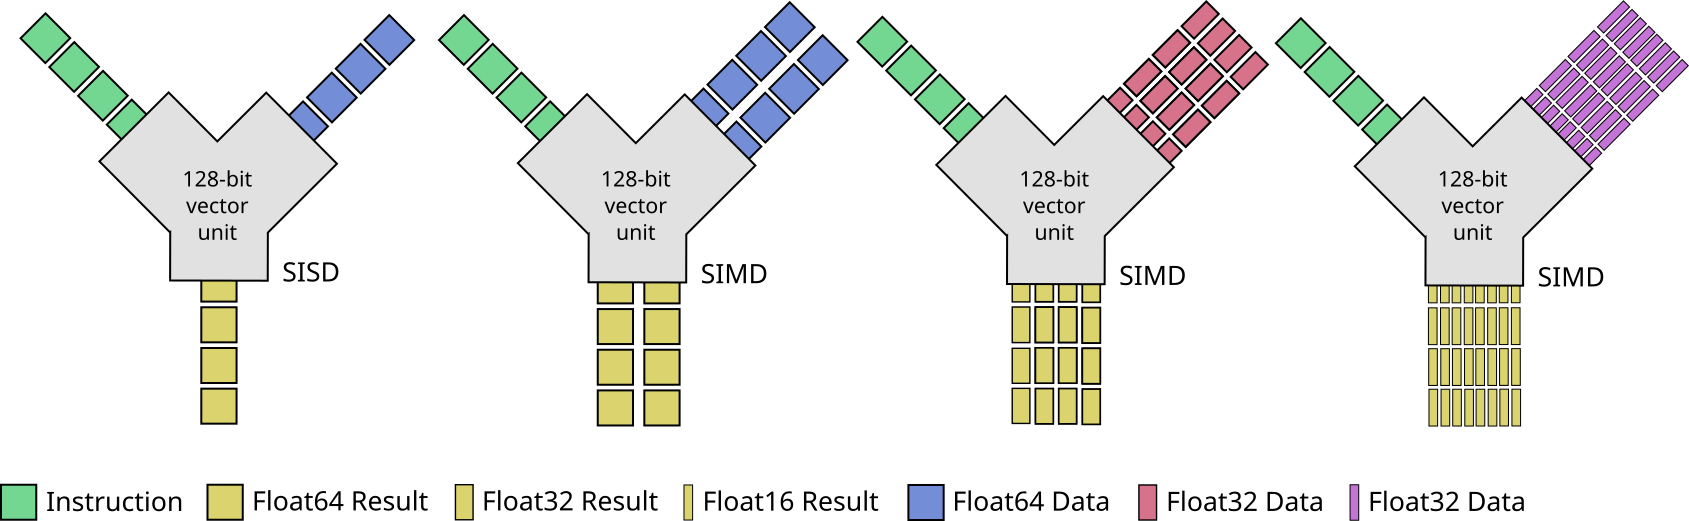
\includegraphics[width=1\textwidth]{Figures/simd.png}
	\caption{Schematic of vector unit operations in single instruction single data and single instruction multiple data configurations with varying precision levels.}
	\label{fig:simd}
\end{figure}
This works as the register is of a fixed size, usually 64-bit, each clock cycle then pushes an instruction to the register where it completes the operation on the data held. If we reduce the bit width of our data to a less precise variable type, i.e. 32 bit, the register is able to perform the same operation on two independent sets of data \cite{banksCALCULATIONENGINEPARAMETERS2014, warneComparisonHighLevel2014, deschryverFPGABasedAccelerators2015}, see diagram in \reffig{fig:simd}. Importantly, it is able to do this in the same clock cycle as if the data had been a single full precision width. This is a key part in how mixed-precision methods can provide significant speed up in high performance computing in lower precision levels \cite{warneVectorOperationsAccelerating2022}. 

Kimpson et al. \cite{kimpsonReducedPrecisionStochasticSimulation2026} investigate methods for computing simulation estimates using mixed and reduced precision in the context of stochastic simulation algorithms (SSAs). These algorithms aim to minimise the error in approximation while using native 16-bit arithmetic. At a hardware-level, this reduces the memory footprint while increasing the SIMD operations able to be computed. They specifically target GPU and tensor processing unit (TPU), which provides insight into how methods can be mapped between device hardware and the results they can achieve in heterogeneous environments. 

\subsection{Reconfigurable Computing}
Reconfigurable computing is classified by a computer architecture that is able to change its logic programming \cite{warneVectorOperationsAccelerating2022}. The most common and popular example of which are FPGAs, built from 'reconfigurable fabric' which contains the configurable logic blocks, interconnections and BRAM that allow the hardware to change its logic functions \cite{cardosoChapter2Highperformance2017}. Essentially, we can create reconfigurable circuitry at the logic-gate level, which gives the user the ability to accurately approximate the functions of a printed circuit board. 

In computing, this means that we are able to construct programs not at a software level, but instead program them onto the architecture of the card. This is a key aspect of the power efficiency that these devices can provide. Unlike CPUs and GPUs, they have a significantly reduced overhead power cost related to unnecessary and always-active processes. 

These devices have been traditionally used by electrical engineers for hardware prototyping and development, requiring users to understand low-level hardware description languages (HDLs). Hence, making them inaccessible to scientific researchers without the proper background to fully take advantage of their utility. Recent advancements in compilation software have lead to the ability for portable programming languages --- OpenCL, HLS, and others --- to be compiled into bit-stream, meaning they are now able to be used to program these devices. This has made them a target of active research in areas such as high-dimensional linear algebra \cite{warneComparisonHighLevel2014,ComparingEnergyEfficiency, macintoshImplementationParallelTridiagonal2016, macintoshImplementingEvaluatingHeterogeneous2019, warneSolvingTriDiagonalLinear}, simulation problems \cite{banksCALCULATIONENGINEPARAMETERS2014} and time-critical safety operations \cite{warnePulsecoupledNeuralNetwork2014}.

As a result of the freedom provided by FPGA hardware, we are also able to increase computational efficiency in low precision settings through the creation of unique precision levels. Unlike modern GPUs, which can provide either double (64-bit), float (32-bit) or half-precision (16-bit), we are able to define custom bit length precision data types. This can be directly applied in areas such as mixed-precision Multilevel Monte Carlo methods, which optimise the fidelity of simulations while retaining an equivalent output approximation \cite{haasNestedMLMCFramework2025}.

Intelligence processing units (IPUs) are an another emerging technology driven by the need for more specialised Artificial Intelligence computing capabilities \cite{kulkarniAcceleratingSimulationbasedInference2020}. Unlike traditional GPU architecture, which uses single-instruction multiple data (SIMD) vectorised parallelism to accelerate tasks, the IPU utilises multi-instruction multiple data (MIMD) \cite{jiaDissectingGraphcoreIPU2019}. This allows each thread to perform operations in a distinct flow, and irregular data access patterns without loss of efficiency \cite{jiaDissectingGraphcoreIPU2019}. Similarly to FPGAs, these devices are also able to define custom precision data types, which has made them extremely efficient processors in AI inference problems \cite{fitzgibbonStochasticRoundingFew2025,sunIntelligenceProcessingUnits2022,MixedPrecisionArithmeticAI}.

\subsection{Systems Biology}
To contextualise our problem we focus on the topic of systems biology, these models look to capture the complex behaviour of intracellular processes with the goal to better understand the functioning of cells as a whole \cite{abkowitzEvidenceThatHematopoiesis1996, arkinStochasticKineticAnalysis1998, kaernStochasticityGeneExpression2005, wilkinsonStochasticModellingQuantitative2009}. The classical approach to describing biological systems are continuous-time deterministic models \cite{wilkinsonStochasticModellingQuantitative2009,highamModelingSimulatingChemical2008}. Using deterministic models however, fails to explore the intrinsic randomness of biochemical reaction networks, and as such we lose valuable information about the true nature of the system \cite{elowitzStochasticGeneExpression2002,rajNatureNurtureChance2008}. As a result of this, the development of stochastic methods have become popular to capture the variability among genetically identical cells \cite{rajNatureNurtureChance2008}. 

Gene expression and regulation are fundamental applications of stochastic modelling methods in which research aims to understand the processes of cellular reproduction and phenotypic characteristics \cite{kaernStochasticityGeneExpression2005,elowitzStochasticGeneExpression2002}. It is well established that these processes are fundamentally stochastic. The nature of experimental data within whole cell modelling introduces substantial complication in generating and fitting stochastic models \cite{wilkinsonStochasticModellingQuantitative2009}. As such, it is common to instead generate stochastic simulations to produce meaningful data for analysis \cite{sunnakerApproximateBayesianComputation2013,highamModelingSimulatingChemical2008}. 

Within systems biology, a primary computational challenges is the forwards problems \cite{warneSimulationInferenceAlgorithms2019}. This refers to the prediction of future state of a system. Namely we must consider the simulation of sample paths of our biochemical reaction networks over time, and the expectation of average behaviour among all possible reaction events \cite{warneSimulationInferenceAlgorithms2019}. This is where Monte Carlo methods can be used to describe the summary statistics of the system. 

\subsection{Stochastic Simulation Algorithms}
To understand the overall behaviour of biochemical reaction networks (BCRN), we concern ourselves with only the change in population over time of the molecular species \cite{gillespieExactStochasticSimulation1977,highamModelingSimulatingChemical2008, warneSimulationInferenceAlgorithms2019, wilkinsonStochasticModellingQuantitative2009}. We consider a spatially homogeneous system for the purposes of this work \cite{chenStochasticModelingSimulation2017}. Consider a BCRN with the $N$ unique chemical species, that interact according to $M$ distinct chemical reactions. The $j^{\text{th}}$ reaction is denoted by
\begin{equation}
	\sum_{i=1}^{N} \nu_{i,j}^- X_i\rightarrow\sum_{i=1}^{N} \nu_{i,j}^+ X_i,
\end{equation}
where $\nu_{i,j}^-$ and $\nu_{i,j}^+$ are the reactant and product stoichiometries related to the $i^\text{th}$ chemical species in the $j^\text{th}$ reaction. We denote $X_i(t)$ as the copy number, that is the number of molecules in the system, of the $i^{\text{th}}$ chemical species at time $t>0$. This leads to the system state vector, $\mathbf{X}(t) = [X_1(t),...,X_n(t)]^\intercal$
In the event that the $j^\text{th}$ reaction occurs, the instantaneous system update is, $\mathbf{X}(t) = \mathbf{X}(t^-)+\boldsymbol{\nu}_j$, where $\mathbf{X}(t^-)$ is the state of the system immediately preceding time $t$. The stoichiometric vector $\nu_j = \nu_{*,j}^+ + \nu_{*,j}^-$ defines the net change in the system state as a result of the $j^\text{th}$ reaction event.

We set the kinetic rate parameters of the $M$ chemical reactions to be the vector $\boldsymbol{\theta} = [k_1, k_2, \hdots, k_m]$, where the $j^{\text{th}}$ reaction is associated with parameter $k_j$. The occurrence of these reactions are based defined using the probability framework laid out in \cite{gillespieExactStochasticSimulation1977, gillespieChemicalLangevinEquation2000}. For each reaction $j$, we have an associated \textit{propensity function}, $a_j(\mathbf{X}(t) ; \boldsymbol{\theta})$. This gives the probability of reaction $j$ occurring exactly once within the infinitesimal interval $[t,t+\mathrm{d}t)$ to be proportional to $a_j(\mathbf{X}(t) ; \boldsymbol{\theta})$, and $a_0(\mathbf{X}(t) ; \boldsymbol{\theta}) = \sum_{j=1}^{M} a_j(\mathbf{X}(t) ; \boldsymbol{\theta})$ \cite{highamModelingSimulatingChemical2008, warneSimulationInferenceAlgorithms2019}.

\subsection{Monte Carlo Methods}
Monte Carlo methods are a common first step in understanding the average behaviour of observed system states given some known parameter inputs \cite{warneSimulationInferenceAlgorithms2019,wilkinsonStochasticModellingQuantitative2009}. If one were to want to know the expectation of a function $P$ at some time $t$ given an observed state $S$ it is intuitive to think that we can take repeated samples of the system to determine an average behaviour \cite{metropolisMonteCarloMethod1949}. Formally, to approximate $\mathbb{E}[P]$ a Monte Carlo estimator is the average values $P(\mathbf{X}(t))$ for $N$ i.i.d. samples $\mathbf{X}(t)$ 
\begin{equation}
	\mathbb{E}[P(\mathbf{X}(t))] = \int P(\mathbf{x})p(\mathbf{x}) \textrm{d}x,\notag
\end{equation}	
\begin{equation}
	\lim_{N\to\infty}\sum_{n=1}^{N} P(\mathbf{X}(t)^{(n)}) =  \mathbb{E}[P(\mathbf{X}(t))],\notag %^\label{eq:monte_carlo_estimator}
\end{equation}
where $p(\mathbf{x})$ is the probability density function of the random variable $\mathbf{X}(t)$. With variance $V_N = \frac{1}{N} \mathbb{V}[P]$, therefore, in order to achieve a root mean squared error (RMSE) of $\epsilon$ we require $N = \mathcal{O}(\epsilon^{-2})$. This is where the Monte Carlo method becomes computationally unwieldy, as each of these simulations often involves the solution to an It\={o} stochastic differential equation (SDE) or a costly approximation. 
\begin{equation}
	X_i(t) = X_i(0) + \sum_{j=1}^{M} \nu_{i,j} \int_0^t a_j(\mathbf{X}(\eta(s)) ; \boldsymbol{\theta}) \, ds + \sum_{j=1}^{M} \nu_{ij} \int_0^t \sqrt{a_j(\mathbf{X}(\eta(s)) ; \boldsymbol{\theta})} \, dW_j(s), \label{eqn:ItoSDE}
\end{equation}
noting that $X_i(t)$ is the value of a random solution path at some time $t>0$. When computing these estimates, we have a statistical error from the Monte Carlo and a bias introduced by the discretisation of the It\={o} SDE, thus we have, 
\begin{equation*}
	\textrm{MSE} = \textrm{Var} + \textrm{Bias}^2.
\end{equation*}
If we want a RMSE less than $\epsilon$ we need $N = \mathcal{O}(\epsilon^{-2})$. However, we also need $\tau = \mathcal{O}(\epsilon)$ since $\textrm{Bias} = \mathcal{O}(\tau)$ for Euler Maruyama. As a result, the total cost of the estimator is $\mathcal{O}(\epsilon^{-3})$. 

Due to this, we seek methods for generating more accurate results while minimising the number of Monte Carlo samples we need to take. Methods such as quasi-Monte Carlo in which each sample is chosen deterministically to reduce the error \cite{dickHighdimensionalIntegrationQuasiMonte2013}. An alternative, the multilevel Monte Carlo method, uses a coupling scheme to apply \textit{control variate reduction} to minimise simulation cost for some desired RMSE $\epsilon$. 
